\section{Introduction}
The use of dynamic reconstruction has been proposed and shown to improve noise ans bias of estimates for parametric imaging etc.

In this chapter we describe the implementation of dynamic reconstruction functionalities in CASToR and the expansions of the framework for reconstruction of DWB datasets. A large fraction of this PhD project was given in the development and validation testing of these functionalities. 
We then show results of dynamic reconstruction applied on the DWB datasets from the IsotoPK study and discuss on potential benefits from the use of a generic dynamic model in exploratory studies such as the IsotoPK. 
Finally we present a novel work conducted towards reduction of kinetic modelling errors using adaptive models is dynamic reconstruction, which was implemented in CASToR and evaluated on IsotoPK study data. 

\section{Methods}

\subsection{Development of dynamic reconstruction framework}
The framework for dynamic reconstruction was developed within the general framework and following the general principles of CASToR, to allow for future expansions including more dynamic models and in order to make our developments publicly available with the public CASToR version. 
To handle use of dynamic models in reconstruction a new component was implemented (called Dynamic-Model-Manager) that interacts with the reconstruction process within the main CASToR iterative loop (steps \textit{Estimate/Fit dynamic model} and \textit{Estimate image from fitted dynamic model} of algorithm~\ref{algo:CASToR_Core}). 
The main tasks of the Dynamic-Model-Manager are to fit dynamic models, given an estimate of a time series of image data, and then estimate the time series image data from the fitted dynamic model. 
As described in section~\ref{section:Fully_4D_reconstruction}, dynamic reconstruction for linear dynamic models can be made using a set of basis functions directly implemented within the system matrix~\cite{Matthews1995,Wang2008,Reader2014}. But as this method results in algorithms with substantially slow overall convergence properties, the nested framework~\cite{Wang2010,Matthews2010} is preferred, which decouples the dynamic model fitting process on image space data from the tomographic update process over the raw PET data.
We have designed the Dynamic-Model-Manager in order to allow for both options of dynamic reconstruction, which we will refer to as non-nested and nested dynamic reconstruction respectively. 
In the examples and evaluations in this project the nested framework was used for practical computational requirements, which is also the method that predominates in most applications of dynamic reconstruction. But the availability of the non-nested option can still be used for comparisons of convergence behaviour and speeds, between non-nested and nested optimization, with new models or on new type of datasets. 

A diagram of the implemented framework for dynamic models is given in figure~\ref{fig3_2:DynamicModelManager}. 
A generic dynamic model (vDynamicModel) was designed, which implements the requirements for model fitting processes, as well as some common optimization algorithms (Least-Squares (LS) and Non-Negative Least-Squares (NNLS) optimization algorithms).
Specific dynamic models can be directly implemented by inheriting these functions from the vDynamicModel class, such as the 1TC and 2TC models in our implementation. These are specific models, based on estimation of micro-parameters of the respective compartmental models, and make use of non-linear optimization of linearization techniques that are unique to these implementations of these models. 
Many models used in practice are linear models and share common optimization methods. For this reason a generic Linear model (iLinearModel) was created, which implements EM optimization (in image space) and allows for the use of LS and NNLS algorithms. The linear model can be used directly, if an input of basis functions is provided. Alternatively specific linear models can be implemented, which can inherit the optimization functions of the generic linear model. These specific linear models need only to define a function for calculating the needed basis functions. 
In our implementation we have implemented two specific linear models, the Patlak model and the spectral analysis model. 
Finally, as most dynamic models that relate to physiological kinetic parameters require information of the blood input function an input function class was created (oArterialInputFunction). This class takes a provided input function and performs linear interpolation of the input data, before providing it for use to the dynamic model. 

\begin{figure} [ht!]
\centering
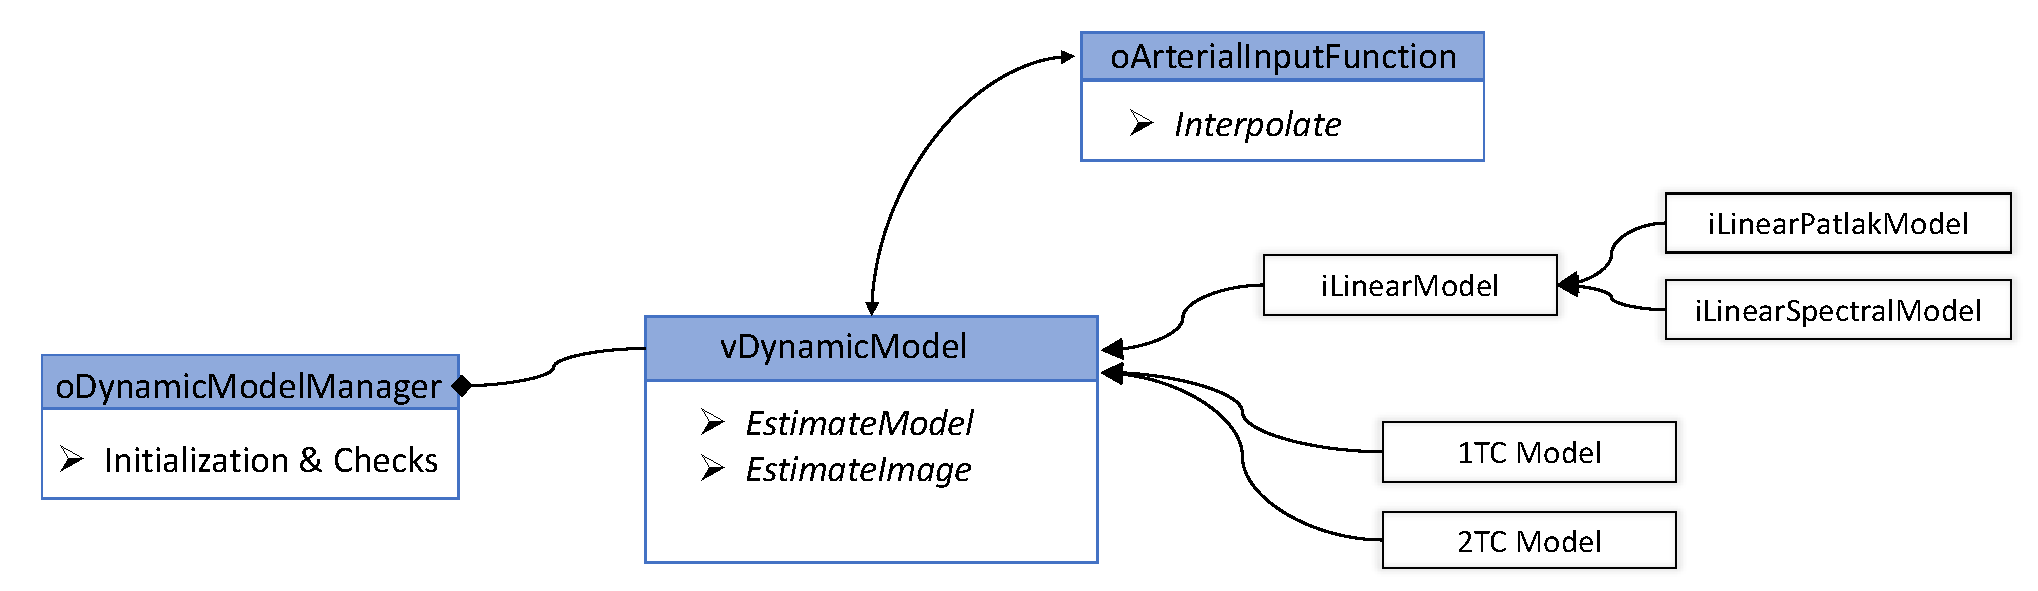
\includegraphics[scale=0.5,angle=0]{3_Results/3_2_DWB_Reconstruction/figures/oDynamicModelManager.pdf}
\caption{CASToR framework for dynamic reconstructions.} 
%TODO: Add over-scan in the CBM DWB protocols. 
\label{fig3_2:DynamicModelManager}
\end{figure}

\subsection{Simulation and demonstration of dynamic reconstruction}
In similar fashion to the design of the dynamic reconstruction framework, a similar approach was used to implemented dynamic models in an in-house developed analytical PET simulator~\cite{Stute2015}. 
The simulator was used to validate the implemented dynamic reconstruction framework and for conducting an simulation study that is presented in the following chapter.

-- Demonstration with 2D Brain
-- Real Data validation and demonstration (H\&N Data ?)